\documentclass[a4paper,fleqn]{article}

\usepackage{fancyhdr}
\usepackage{extramarks}
\usepackage{amsmath}
\usepackage{amsthm}
\usepackage{amsfonts}
\usepackage{tikz}
\usepackage[plain]{algorithm}
\usepackage{algpseudocode}
\usepackage{amsmath}
\usepackage{verbatim}
\usepackage{graphicx}
\usepackage{epstopdf}

\usetikzlibrary{automata,positioning}

%
% Basic Document Settings
%

\topmargin=-0.45in
\evensidemargin=0in
\oddsidemargin=0in
\textwidth=6.5in
\textheight=9.0in
\headsep=0.25in

\linespread{1.1}

\pagestyle{fancy}
\lhead{\hmwkAuthorName}
%\chead{\hmwkClass\ (\hmwkClassInstructor): \hmwkTitle}
\rhead{\hmwkAuthorUNI}
\lfoot{\lastxmark}
\cfoot{\thepage}

\renewcommand\headrulewidth{0.4pt}
\renewcommand\footrulewidth{0.4pt}

\setlength\parindent{0pt}

%
% Create Problem Sections
%

\newcommand{\enterProblemHeader}[1]{
    %\nobreak\extramarks{}{Problem \arabic{#1} continued on next page\ldots}\nobreak{}
    %\nobreak\extramarks{Problem \arabic{#1} (continued)}{Problem \arabic{#1} continued on next page\ldots}\nobreak{}
}

\newcommand{\exitProblemHeader}[1]{
    %\nobreak\extramarks{Problem \arabic{#1} (continued)}{Problem \arabic{#1} continued on next page\ldots}\nobreak{}
    \stepcounter{#1}
    %\nobreak\extramarks{Problem \arabic{#1}}{}\nobreak{}
}

\setcounter{secnumdepth}{0}
\newcounter{partCounter}
\newcounter{homeworkProblemCounter}
\setcounter{homeworkProblemCounter}{1}
\nobreak\extramarks{Problem \arabic{homeworkProblemCounter}}{}\nobreak{}

\newenvironment{homeworkProblem}{
    \section{Problem \arabic{homeworkProblemCounter}}
    \setcounter{partCounter}{0}
    \enterProblemHeader{homeworkProblemCounter}
}{
    \exitProblemHeader{homeworkProblemCounter}
}

%
% Homework Details
%   - Title
%   - Due date
%   - Class
%   - Section/Time
%   - Instructor
%   - Author
%

\newcommand{\hmwkTitle}{Homework\ \#1}
\newcommand{\hmwkDueDate}{September 18, 2017}
\newcommand{\hmwkClass}{LINEAR REGRESSION MODELS}
%\newcommand{\hmwkClassTime}{Section 005}
\newcommand{\hmwkClassInstructor}{Professor Jingchen Liu}
\newcommand{\hmwkAuthorName}{Fan Yang}
\newcommand{\hmwkAuthorUNI}{UNI: fy2232}

%
% Title Page
%

\title{
    \vspace{2in}
    \textmd{\textbf{\hmwkClass:\ \hmwkTitle}}\\
    \normalsize\vspace{0.1in}\small{Due\ on\ \hmwkDueDate}\\
    \vspace{0.1in}\large{\textit{\hmwkClassInstructor}}
    \vspace{3in}
}

\author{\textbf{\hmwkAuthorName}\\
    \text{\hmwkAuthorUNI}}
\date{}

\renewcommand{\part}[1]{\textbf{\large Part \Alph{partCounter}}\stepcounter{partCounter}\\}

%
% Various Helper Commands
%

% Useful for algorithms
\newcommand{\alg}[1]{\textsc{\bfseries \footnotesize #1}}

% For derivatives
\newcommand{\deriv}[1]{\frac{\mathrm{d}}{\mathrm{d}x} (#1)}

% For partial derivatives
\newcommand{\pderiv}[2]{\frac{\partial}{\partial #1} (#2)}

% Integral dx
\newcommand{\dx}{\mathrm{d}x}

% Alias for the Solution section header
\newcommand{\solution}{\textbf{\large Solution}}

% Probability commands: Expectation, Variance, Covariance, Bias
\newcommand{\E}{\mathrm{E}}
\newcommand{\Var}{\mathrm{Var}}
\newcommand{\Cov}{\mathrm{Cov}}
\newcommand{\Bias}{\mathrm{Bias}}

\begin{document}

\maketitle
\setcounter{page}{0}
\thispagestyle{empty}

\pagebreak

\begin{homeworkProblem}     %1

    \textbf{a.}
    \[
        \begin{split}
            &\widehat{\beta}_1=\frac{\sum(x_i-\overline{x})(y_i-\overline{y})}{(x_i-\overline{x})^2}
            \\
            &\overline{x}=\sum x_i =22.5\\
            &\overline{y}=\sum y_i =3.380\\
            &\widehat{\beta}_1=\frac{\sum(x_i-22.5)(y_i-3.380)}{(x_i-22.5)^2}\\
            &=\frac{7.562}{207.5}=0.036\\
            &\widehat{\beta}_0=\overline{y}-\widehat{\beta}_1*\overline{x}
            =3.380-0.036*22.5=2.560\\
            &therefore~y=2.560+0.036x
            \\
        \end{split}
    \]

    \textbf{b.}

    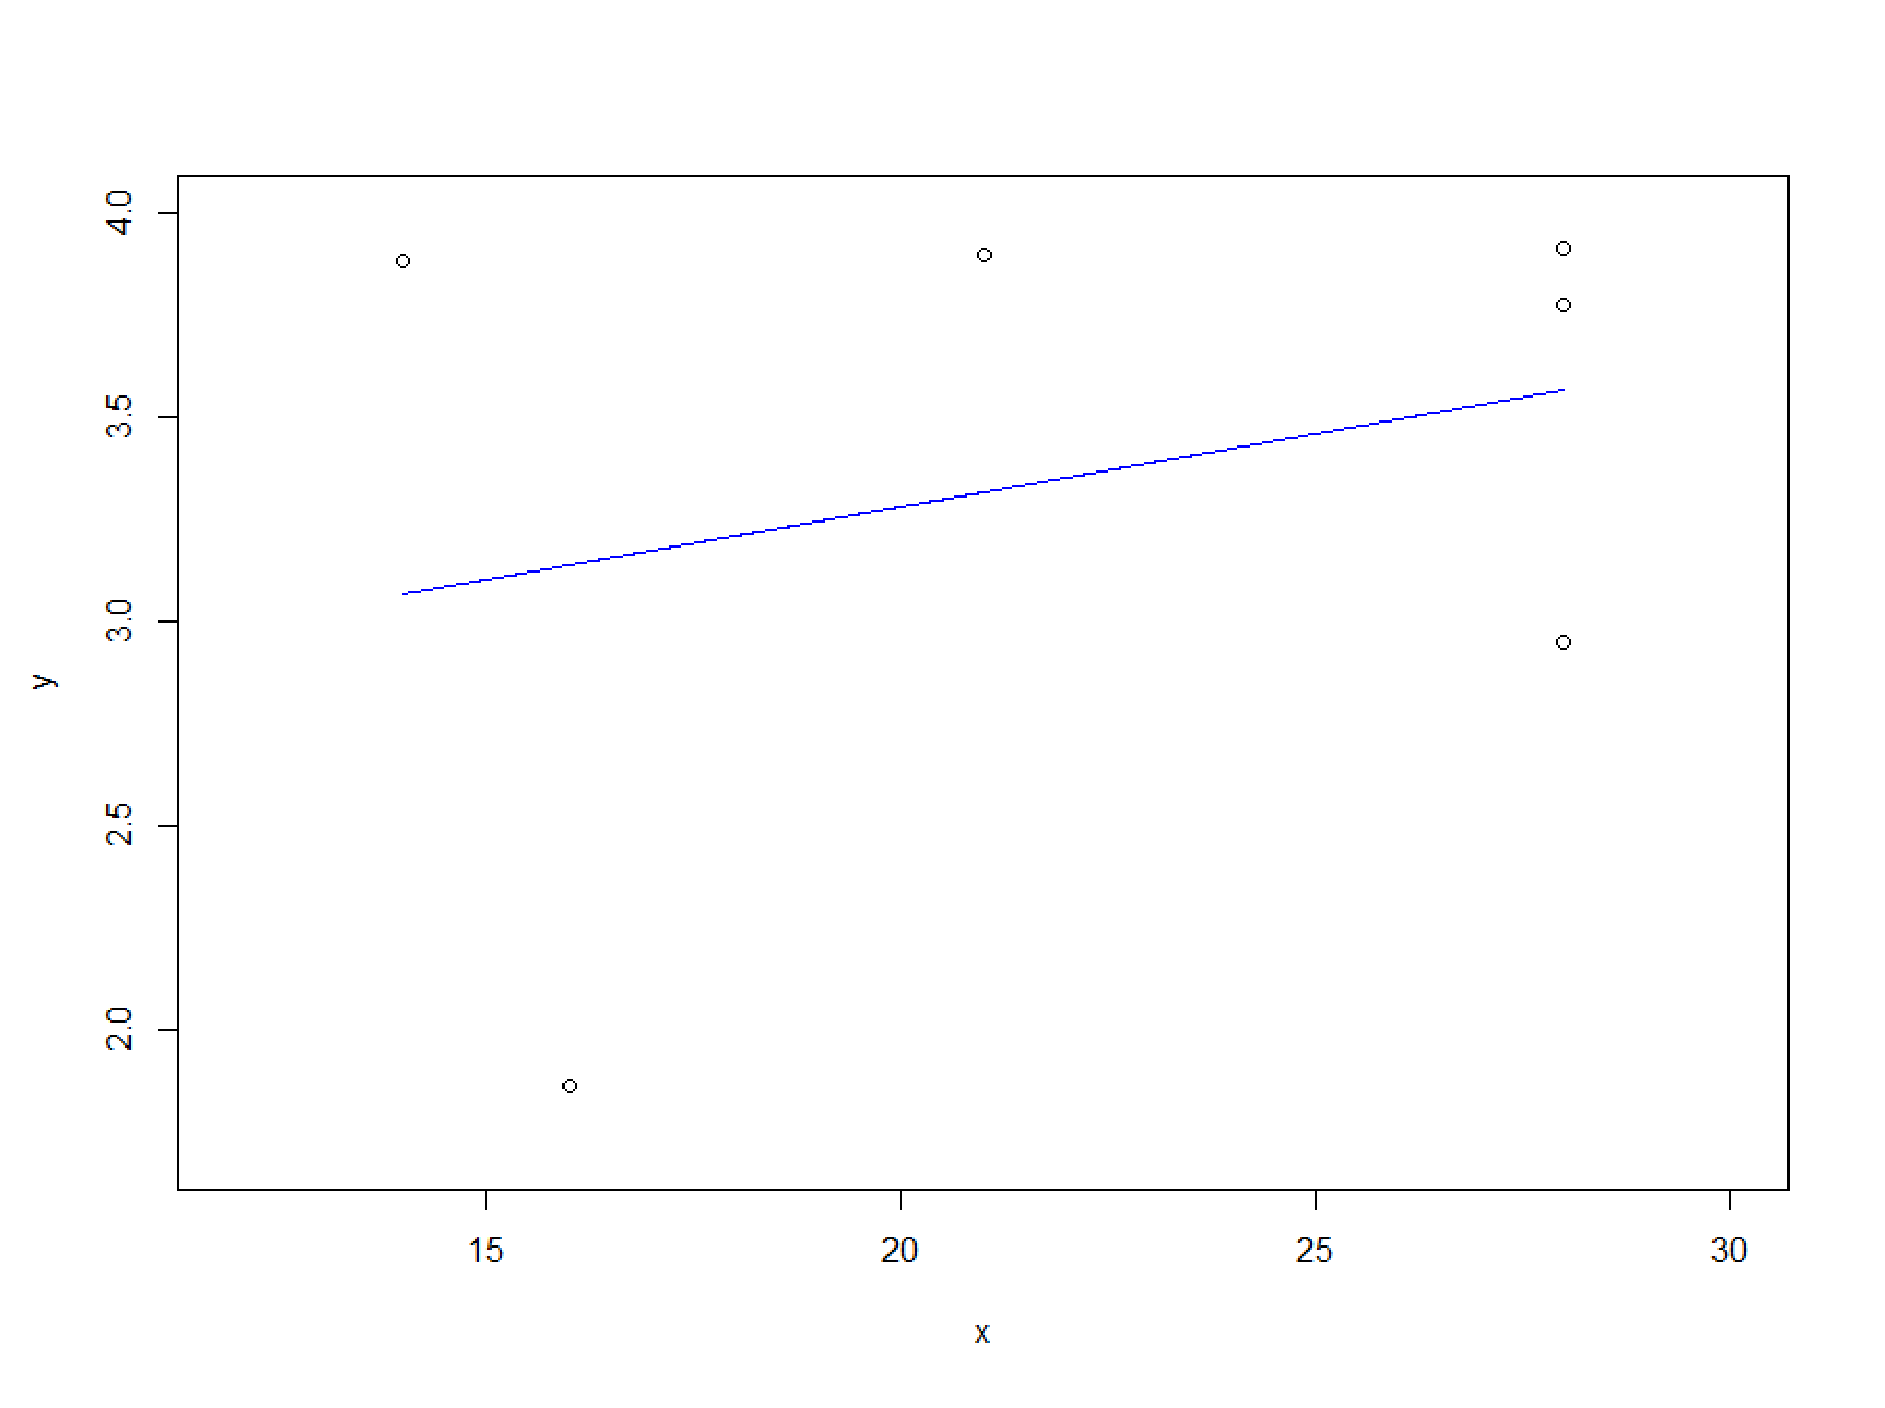
\includegraphics[height=4in]{reg_hw1_pic1}

    \[
        \begin{split}
            &\text{when x=28, there are 3 possible y. so x and y are likely uncorrelated. }\\
            &\text{We can draw conclusion from the plot above that the function does not fit the data.}
        \end{split}
    \]
    \textbf{c.}

    \[
        \begin{split}
            \widehat{y}&=\beta_0+\beta_1*x\\
            &=2.560+0.036*30=3.64
        \end{split}
    \]

    \textbf{d.}

    \[
        \begin{split}
            \Delta y=&y_1-y_2=(2.560+0.036*x)-(2.560+0.036*(x+1))=0.036
        \end{split}
    \]

\end{homeworkProblem}

\begin{homeworkProblem}%2

    \[
        \begin{split}
            &\text{When $\beta_0$ is 0,we know that the regression model only determines by $\beta_1$,and the function line goes}\\
            &\text{through origin the point and is a linear line which only depends on the slope.}\\
        \end{split}
    \]

\end{homeworkProblem}

\begin{homeworkProblem}     %3

    \[
        \begin{split}
            &\text{When $\beta_1$ is 0,the response variable is a constant and no longer related to explanatory variable.}\\
            &\text{which means $\beta_0$,and the function line goes through origin the point and is a linear line which}\\
            &\text{only depends on the slope.}\\
        \end{split}
    \]

\end{homeworkProblem}

\begin{homeworkProblem}     %4
    \[
        \begin{split}
    &\text{the goal of least squares estimator is to minimize}\sum_i^n (y_i-\beta_0)^2\\
    &\sum_i^n (y_i-\beta_0)^2=\sum_i^n (y_i-\overline{y}+\overline{y}-\beta_0)^2
    =\sum_i^n (y_i-\overline{y})^2-2\sum_i^n (y_i-\overline{y})(\overline{y}-\beta_0)+\sum_i^n (\overline{y}-\beta_0)^2\\
    &=\sum_i^n (y_i-\overline{y})^2+\sum_i^n (\overline{y}-\beta_0)^2\\
    &\text{in order to minimize the above statement, $\beta_0$ should be equal to $\overline{y}$.}\\
    &\text{Therefore,least squares estimator of $\beta_0$ is }\widehat{\beta_0}=\overline{y}\\
        \end{split}
    \]
\end{homeworkProblem}

\begin{homeworkProblem}     %5

    \[
        \begin{split}
        E(\widehat{\beta}_0)&=E(\overline{y})=E(\frac{1}{n}\sum y_i)\\
        &=\frac{1}{n}E(\sum y_i)=\frac{1}{n}\sum E( y_i)=\frac{1}{n}\sum E(\beta_0)
        =\frac{1}{n}*n*\beta_0\\
        &=\beta_0\\
        \text{so that $\widehat{\beta}_0$ is unbiased}\\
        \end{split}
    \]


\end{homeworkProblem}

\begin{homeworkProblem}     %6

    \textbf{a.}
    \[
        \begin{split}
        &\text{We use the following conclusion without proof}\\
        &\widehat{\beta}_1=\frac{\sum(x_i-\overline{x})(y_i-\overline{y})}{(\sum x_i-\overline{x})^2}\\
        &\widehat{\beta}_0=\overline{y}-\widehat{\beta}_1 \overline{x}\\
        &\overline{x}=10\\
        \\
        &\text{denote $\overline{Y}$ as the mean of the 6 observations( also the mean of 3 means of observations)}\\
        &\text{1) in the 3 points regression}\\
        &\widehat{\beta}_1^1=\frac{(5-10)(\overline{Y}_1-\overline{Y})+(10-10)(\overline{Y}_2-\overline{Y})+(15-10)(\overline{Y}_3-\overline{Y})}
        {(5-10)^2+(10-10)^2+(15-10)^2}\\
        &=\frac{5(\overline{Y}_1-\overline{Y})+5(\overline{Y}_3-\overline{Y})}{50}
        =\frac{(\overline{Y}_1-\overline{Y})+(\overline{Y}_3-\overline{Y})}{10}\\
        \\
        &\text{2) in the 6 points regression}\\
        &\widehat{\beta}_1^2=\frac{(5-10)[(Y_{11}-\overline{Y})+(Y_{12}-\overline{Y})]
        +(10-10)[(Y_{21}-\overline{Y})+(Y_{22}-\overline{Y})]
        +(15-10)[(Y_{32}-\overline{Y})+(Y_{33}-\overline{Y})]}
        {2*(5-10)^2+2*(10-10)^2+2*(15-10)^2}\\
        &=\frac{5(Y_{11}-\overline{Y}+Y_{12}-\overline{Y})+5(Y_{31}-\overline{Y}+Y_{32}-\overline{Y})}{100}\\
        &=\frac{5(2\overline{Y}_1-2\overline{Y})+5(2\overline{Y}_3-2\overline{Y})}{100}\\
        &=\frac{(\overline{Y}_1-\overline{Y})+(\overline{Y}_3-\overline{Y})}{10}\\
        &=\widehat{\beta}_1^1\\
        \\
        &\text{that's to say, the $\widehat{\beta}_1$ in two models are identical}\\
        &\text{Besides, $\overline{X}$ and $\overline{Y}$ are same in two models.}\\
        &\text{according to $\widehat{\beta}_0=\overline{y}-\widehat{\beta}_1 \overline{x}$ we know $\widehat{\beta}_0$ are same.}\\
        &\text{therefore, the two regression lines are identical.}
        \end{split}
    \]

    \textbf{b.}

    \[
        \begin{split}
        &s^2=MSE=\frac{SSE}{n-2}=\frac{\sum(Y_i-\widehat{Y}_i)^2}{n-2}\\
        &E(MSE)=\sigma^2\\
        \end{split}
    \]

\end{homeworkProblem}


\begin{homeworkProblem}     %7
    
    \textbf{a.}
    
    \[
        \begin{split}
        &\text{We use the following conclusion without proof}\\
        &\widehat{\beta}_1=\frac{\sum(x_i-\overline{x})(y_i-\overline{y})}{(\sum x_i-\overline{x})^2}\\
        &\widehat{\beta}_0=\overline{y}-\widehat{\beta}_1 \overline{x}\\
        &\text{since we know that $\beta_0=0$ }\\
        &\text{then }0=\overline{y}-\widehat{\beta}_1 \overline{x}\\
        &\overline{y}=\widehat{\beta}_1 \overline{x}\\
        \end{split}
    \]
    
    \textbf{b.}

    \[
        \begin{split}
        &\varepsilon_i\sim N(0,\sigma^2),pdf=\frac{1}{\sigma \sqrt{2\pi}}exp\left(-\frac{x^2}{2\sigma^2}\right)\\
        &L(\beta_1,\sigma)=\prod \limits_{i}^{n} \frac{1}{\sigma \sqrt{2\pi}}exp\left(-\frac{(Y_i-\beta_1X_i)^2}{2\sigma^2}\right)\\
        &=\frac{1}{(\sigma \sqrt{2\pi})^n} exp\left(-\frac{\sum\limits_{i}^{n} (Y_i-\beta_1X_i)^2}{2\sigma^2}\right)\\
        &\text{in order to maximize $L(\beta_1,\sigma)$, we simply only need to minimize $\sum\limits_{i}^{n} (Y_i-\beta_1X_i)^2$}\\
        &\text{now it becomes the same problem as least square estimate,therefore the two estimator of $\beta_1$ are identical.}\\
        &\widehat{\beta}_1=\frac{\sum\limits _i^n(x_i-\overline{x})(y_i-\overline{y})}{\sum\limits _i^n(x_i-\overline{x})^2}\\
        \end{split}
    \]
    
    \textbf{c.}

    \[
        \begin{split}
        &\widehat{\beta}_1=\frac{\sum\limits _i^n(x_i-\overline{x})(y_i-\overline{y})}{\sum\limits _i^n(x_i-\overline{x})^2}\\
        &E(\widehat{\beta}_1)=E(\frac{\sum\limits _i^n(x_i-\overline{x})(y_i-\overline{y})}{\sum\limits _i^n(x_i-\overline{x})^2})
        =\frac{\sum\limits _i^n(x_i-\overline{x})E(y_i-\overline{y})}{\sum\limits _i^n(x_i-\overline{x})^2}
        =\frac{\sum\limits _i^n(x_i-\overline{x})(E(y_i)-\overline{y})}{\sum\limits _i^n(x_i-\overline{x})^2}\\
        &\text{because }E(y_i)=\beta_1x_i~~and~~ \overline{y}=\beta_1x_i~;\\
        &E(\widehat{\beta}_1)=\frac{\sum\limits _i^n(x_i-\overline{x})(\beta_1x_i-\overline{y})}{\sum\limits _i^n(x_i-\overline{x})^2}
        =\frac{\sum\limits _i^n(x_i-\overline{x})(\beta_1x_i-\beta_1\overline{x})}{\sum\limits _i^n(x_i-\overline{x})^2}
        =\frac{\beta_1\sum\limits _i^n(x_i-\overline{x})(x_i-\overline{x})}{\sum\limits _i^n(x_i-\overline{x})^2}\\
        &=\beta_1\\
        &\text{therefore $\widehat{\beta}_1$ is unbiased.}\\
        \end{split}
    \]

\end{homeworkProblem}

\begin{homeworkProblem}     %8

    \textbf{(1)}
    \[
        \begin{split}
        &Pr(agree)=p*p+(1-p)*(1-p)=2p^2-2p+1\\
        &\text{from problem 7 we know }Pr(correct)=p\\
        &Pr(correct|agree)=\frac{Pr(correct\cap agree)}{Pr(agree)}
        =\frac{p*p}{2p^2-2p+1}=\frac{9}{13}\\
        \end{split}
    \]

    \textbf{(2)}
    \[
        \begin{split}
        &Pr(disagree)=p*(1-p)+(1-p)*p=2p(1-p)\\
        &Pr(correct\cap disagree)=\frac{1}{2}*p*(1-p)+\frac{1}{2}(1-p)*p=p(1-p)\\
        &Pr(correct|disagree)=\frac{Pr(correct\cap disagree)}{Pr(disagree)}
        =\frac{p(1-p)}{2p(1-p)}=\frac{1}{2}\\
        \end{split}
    \]

\end{homeworkProblem}

\begin{homeworkProblem}     %9
    \[
        \begin{split}
        &\text{we will calculate the chance that there is no head}\\
        &Pr_{(no~head)}=(1-p)^n.\\
        &\text{in contrast, the probability that at least one head is}\\
        &Pr_{(at~least~one~head)}=1-(1-p)^n\\
        &1-(1-p)^n\geq 0.5\Leftrightarrow (1-p)^n\leq 0.5\\
        &1-p\in [0,1];~so~n*log(1-p)\leq log(0.5)\\
        &\Leftrightarrow n\geq \frac{log(\frac{1}{2})}{log(1-p)}\\
        &\text{and p could not equal to 1}\\
        \end{split}
    \]

\end{homeworkProblem}

\begin{homeworkProblem}     %10
    \[
        \begin{split}
        &\text{denote the event a silver coin is found as E}\\
        &Pr(E)=\frac{1}{3}*\frac{1}{2}+\frac{1}{3}*1=\frac{1}{2}\\
        &\text{denote the event two silver coins ia found as F}\\
        &Pr(F)=\frac{1}{3}\\
        &Pr(F|E)=\frac{Pr(F\cap E)}{Pr(E)}\\
        &=\frac{Pr(F)}{Pr(E)}=\frac{\frac{1}{3}}{\frac{1}{2}}=\frac{2}{3}\\
        \end{split}
    \]

\end{homeworkProblem}

\begin{homeworkProblem}     %11

    \textbf{(a)}
    \[
        \begin{split}
        &\text{let's separate this event into two parts:}\\
        &\text{a)a red ball is drawn from A; b)any ball other than red is drawn form A}\\
        &then~P=\frac{4}{4+3+2}*\frac{3}{3+3+4}
        +\frac{3+2}{4+3+2}*\frac{2}{2+3+4+1}
        =\frac{11}{45}\\
        \end{split}
    \]

    \textbf{(b)}

    \[
        \begin{split}
        &\text{denote E as drawn red from A and F as drawn red from B}\\
        &\text{from part (a) we get}~ Pr(F)=\frac{11}{45}\\
        &Pr(E\cap F)=\frac{4}{4+3+2}*\frac{3}{3+3+4}=\frac{2}{15}\\
        &Pr(E|F)=\frac{Pr(E\cap F)}{Pr(F)}\\
        &=\frac{Pr(E\cap F)}{Pr(F)}=\frac{\frac{2}{15}}{\frac{11}{45}}
        =\frac{6}{11}\\
        \end{split}
    \]

\end{homeworkProblem}

\begin{homeworkProblem}     %12 #7 on page 21

    %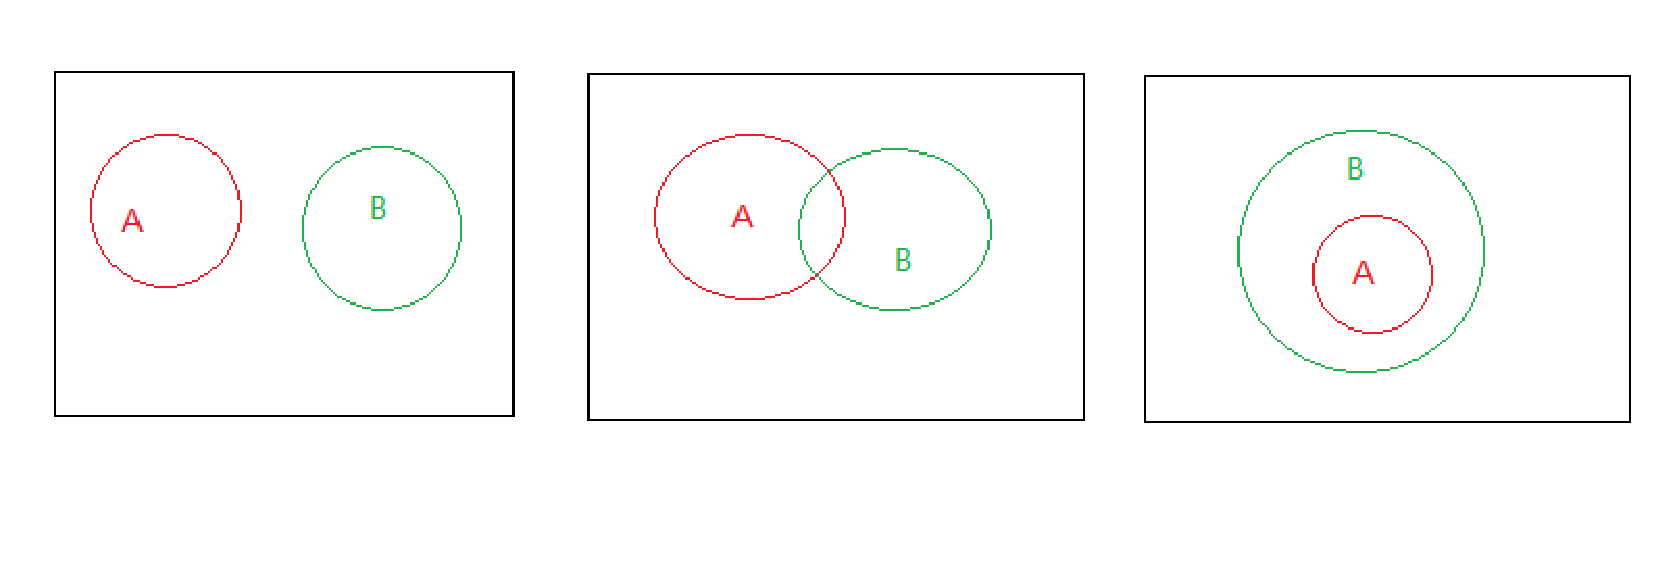
\includegraphics[height=2in]{prob_hw1_pic1}

    \[
        \begin{split}
        &\text{from the above venn  diagram,we come to the following conclusion:}\\
        &\text{1) when A and B are independent, then}~Pr(A\cap B)~\text{get the minimum value 0.}\\
        &\text{2) when B is a sub set of A, then}~Pr(A\cap B)~\text{get the maximum value 0.7.}\\
        \end{split}
    \]

\end{homeworkProblem}

\begin{homeworkProblem}     %13    #3 on page 25.

    %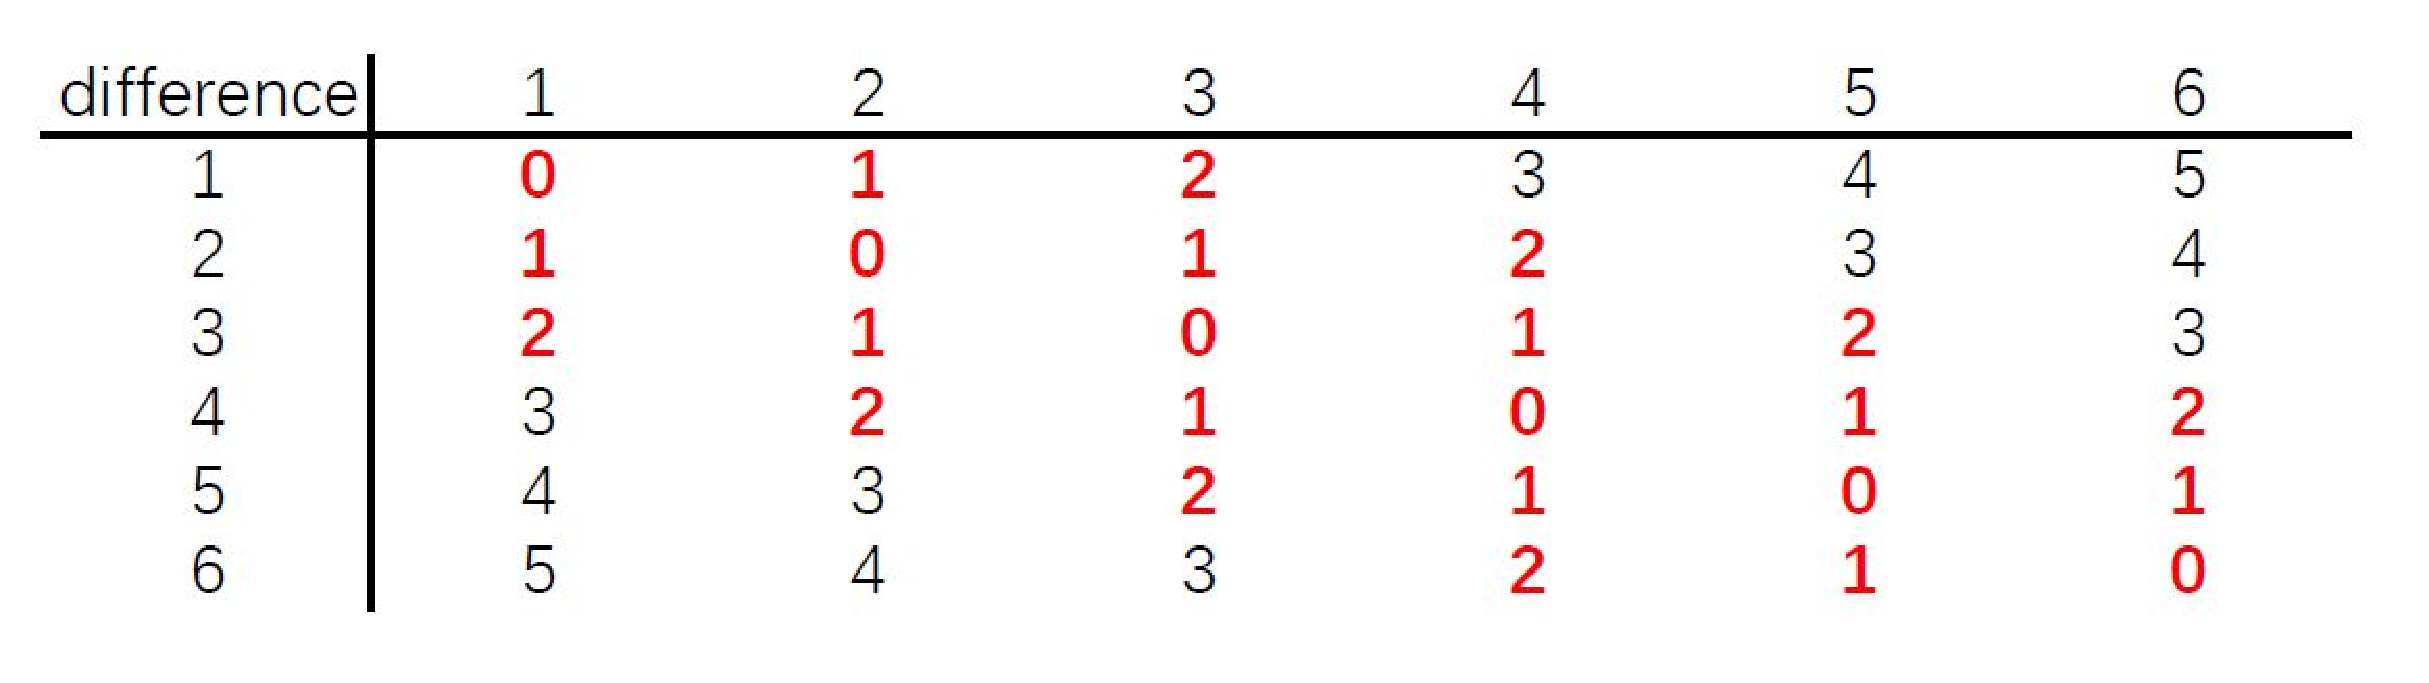
\includegraphics[height=1.5in]{prob_hw1_pic2}

    \[
        \begin{split}
        &\text{as the graph above depicts, we get:}\\
        &P=\frac{24}{36}=\frac{2}{3}\\
        \end{split}
    \]

\end{homeworkProblem}

\begin{homeworkProblem}     %14    #7 on page 32.
    \[
        \begin{split}
        &\text{the number in sample space should be}
        \left(\begin{array}{c}12+20-1\\12 \end{array} \right)
        =\left(\begin{array}{c}31\\12 \end{array} \right)\\
        &\text{the situation that no box have more than one ball is the same as there are}\\
        &\text{ 12 boxes with one box each only and 8 empty boxes}\\
        &\text{so number of choices of this situation is }
        \left(\begin{array}{c}20\\12\end{array}\right)\\
        &therefore~P=\frac{\left(\begin{array}{c}20\\12\end{array}\right)}
        {\left(\begin{array}{c}31\\12\end{array}\right)}\\
        &=\frac{646}{723695}\\
        \end{split}
    \]

\end{homeworkProblem}

\begin{homeworkProblem}     %15    #12 on page 41
    \[
        \begin{split}
        &\text{the number in sample space should be}
        \left(\begin{array}{c}35\\10 \end{array} \right)\\
        &\text{number of choices of this situation is }
        \left(\begin{array}{c}35-2\\10-2\end{array}\right)+
        \left(\begin{array}{c}35-2\\10\end{array}\right)\\
        &=\left(\begin{array}{c}33\\8\end{array}\right)+
        \left(\begin{array}{c}33\\10\end{array}\right)\\
        &so~P=\frac{\left(\begin{array}{c}33\\8\end{array}\right)+
        \left(\begin{array}{c}33\\10\end{array}\right)}{\left(\begin{array}{c}35\\10 \end{array} \right)}\\
        &=\frac{69}{119}\\
        \end{split}
    \]

\end{homeworkProblem}

\begin{homeworkProblem}     %16    #8 on page 46.
    \[
        \begin{split}
        &\text{the number in sample space should be}
        \left(\begin{array}{c}52\\13,13,13,13 \end{array} \right)\\
        &\text{number of choices of this situation is }
        \left(\begin{array}{c}12\\3,3,3,3\end{array}\right)*
        \left(\begin{array}{c}40\\10,10,10,10\end{array}\right)\\
        &so~P=\frac{\left(\begin{array}{c}12\\3,3,3,3\end{array}\right)*
        \left(\begin{array}{c}40\\10,10,10,10\end{array}\right)}
        {\left(\begin{array}{c}52\\13,13,13,13 \end{array} \right)}\\
        &=\frac{\frac{12!}{(3!)^4}*\frac{40!}{(10!)^4}}{\frac{52!}{(13!)^4}}\\
        &=\frac{\frac{12!}{(3!)^4}*\frac{40!}{(10!)^4}}{\frac{52!}{(13!)^4}}\\
        &=\frac{148933}{4594023}\approx 0.0324
        \end{split}
    \]

\end{homeworkProblem}

\begin{homeworkProblem}     %17    #6 on page 50.
    \[
        \begin{split}
        &\text{the number in sample space should be}
        \left(\begin{array}{c}30*3\\10 \end{array} \right)\\
        &\text{number of choices of missing one color is }
        \left(\begin{array}{c}30*2\\10\end{array}\right)-2*
        \left(\begin{array}{c}30\\10\end{array}\right)\\
        &\text{number of choices of missing two color is }
        3*\left(\begin{array}{c}30\\10\end{array}\right)\\
        &so~P=\frac{\left(\begin{array}{c}30*2\\10\end{array}\right)-2*
        \left(\begin{array}{c}30\\10\end{array}\right)
        +3*\left(\begin{array}{c}30\\10\end{array}\right)}
        {\left(\begin{array}{c}30*3\\10 \end{array} \right)}\\
        &=\frac{9734}{738289}\approx 0.0132
        \end{split}
    \]

\end{homeworkProblem}

\end{document}
